\documentclass[11pt]{article}
\usepackage[margin=1.6cm]{geometry}
\usepackage{amsmath,xcolor,graphicx,tikz,needspace}
\usetikzlibrary{decorations.pathreplacing}
\setlength{\parindent}{0pt}
\begin{document}
\begin{center}{\LARGE BraidTeX Composition Gallery}\end{center}
\small This gallery is generated from the public BraidTeX model API. The diagrams use model-level stacking, cabling substitution, persistent strand identities, and separate topological and annotation primitives.
\medskip
\needspace{6.3cm}
\textbf{Smooth shifts and an exchange}\par
\smallskip
\begin{center}\resizebox{!}{5.0cm}{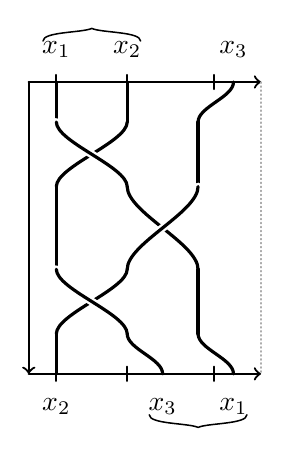
\begin{tikzpicture}[x=1cm,y=1cm,line cap=round,line join=round]
\coordinate (braid-base) at (1.125,-0.5084);
\draw[draw=black,line width=0.8pt,->] (-0.35,3.1984) -- (2.6,3.1984);
\draw[draw=black,line width=0.8pt,->] (-0.35,-0.5084) -- (2.6,-0.5084);
\draw[draw=black,line width=0.8pt,->] (-0.35,3.1984) -- (-0.35,-0.5084);
\draw[gray!65,densely dotted,line width=0.45pt] (2.6,3.1984) -- (2.6,-0.5084);
\draw[draw=black,line width=0.8pt] (0,3.1084) -- (0,3.2884);
\draw[draw=black,line width=0.8pt] (0.9,3.1084) -- (0.9,3.2884);
\draw[draw=black,line width=0.8pt] (2,3.1084) -- (2,3.2884);
\draw[draw=black,line width=0.8pt] (0,-0.5984) -- (0,-0.4184);
\draw[draw=black,line width=0.8pt] (0.9,-0.5984) -- (0.9,-0.4184);
\draw[draw=black,line width=0.8pt] (2,-0.5984) -- (2,-0.4184);
\draw[draw=black,line width=1.15pt] (0,3.1984) .. controls (0,3.00521) and (0,2.88319) .. (0,2.69);
\draw[draw=black,line width=1.15pt] (0.9,3.1984) .. controls (0.9,3.00521) and (0.9,2.88319) .. (0.9,2.69);
\draw[draw=black,line width=1.15pt] (2.25,3.1984) .. controls (2.25,3.00521) and (1.8,2.88319) .. (1.8,2.69);
\draw[draw=black,line width=1.15pt] (1.8,2.69) -- (1.8,1.87);
\draw[draw=black,line width=1.15pt] (0.9,2.69) .. controls (0.9,2.4358) and (0,2.1242) .. (0,1.87);
\draw[draw=white,line width=2.85pt] (0,2.69) .. controls (0,2.4358) and (0.9,2.1242) .. (0.9,1.87);
\draw[draw=black,line width=1.15pt] (0,2.69) .. controls (0,2.4358) and (0.9,2.1242) .. (0.9,1.87);
\draw[draw=black,line width=1.15pt] (0,1.87) -- (0,0.82);
\draw[draw=black,line width=1.15pt] (0.9,1.87) .. controls (0.9,1.5445) and (1.8,1.1455) .. (1.8,0.82);
\draw[draw=white,line width=2.85pt] (1.8,1.87) .. controls (1.8,1.5445) and (0.9,1.1455) .. (0.9,0.82);
\draw[draw=black,line width=1.15pt] (1.8,1.87) .. controls (1.8,1.5445) and (0.9,1.1455) .. (0.9,0.82);
\draw[draw=black,line width=1.15pt] (1.8,0.82) -- (1.8,0);
\draw[draw=black,line width=1.15pt] (0.9,0.82) .. controls (0.9,0.5658) and (0,0.2542) .. (0,0);
\draw[draw=white,line width=2.85pt] (0,0.82) .. controls (0,0.5658) and (0.9,0.2542) .. (0.9,0);
\draw[draw=black,line width=1.15pt] (0,0.82) .. controls (0,0.5658) and (0.9,0.2542) .. (0.9,0);
\draw[draw=black,line width=1.15pt] (0,0) .. controls (0,-0.19319) and (0,-0.31521) .. (0,-0.5084);
\draw[draw=black,line width=1.15pt] (0.9,0) .. controls (0.9,-0.19319) and (1.35,-0.31521) .. (1.35,-0.5084);
\draw[draw=black,line width=1.15pt] (1.8,0) .. controls (1.8,-0.19319) and (2.25,-0.31521) .. (2.25,-0.5084);
\node[inner sep=1pt,anchor=south] at (0,3.4684) {$x_1$};
\node[inner sep=1pt,anchor=south] at (0.9,3.4684) {$x_2$};
\node[inner sep=1pt,anchor=south] at (2.25,3.4684) {$x_3$};
\node[inner sep=1pt,anchor=north] at (0,-0.7784) {$x_2$};
\node[inner sep=1pt,anchor=north] at (1.35,-0.7784) {$x_3$};
\node[inner sep=1pt,anchor=north] at (2.25,-0.7784) {$x_1$};
\draw[line width=0.55pt] (-0.17,3.7184) .. controls (-0.17,3.8384) and (0.326,3.8224) .. (0.45,3.8784) .. controls (0.574,3.8224) and (1.07,3.8384) .. (1.07,3.7184);
\draw[line width=0.55pt] (1.18,-1.0284) .. controls (1.18,-1.1484) and (1.676,-1.1324) .. (1.8,-1.1884) .. controls (1.924,-1.1324) and (2.42,-1.1484) .. (2.42,-1.0284);
\end{tikzpicture}
}\end{center}
\smallskip
\needspace{6.3cm}
\textbf{A connector with only its endpoint nodes}\par
\smallskip
\begin{center}\resizebox{!}{5.0cm}{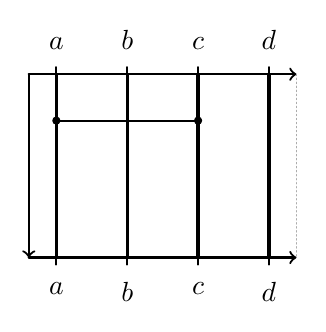
\begin{tikzpicture}[x=1cm,y=1cm,line cap=round,line join=round]
\coordinate (braid-base) at (1.35,-0.589);
\draw[draw=black,line width=0.8pt,->] (-0.35,1.739) -- (3.05,1.739);
\draw[draw=black,line width=0.8pt,->] (-0.35,-0.589) -- (3.05,-0.589);
\draw[draw=black,line width=0.8pt,->] (-0.35,1.739) -- (-0.35,-0.589);
\draw[gray!65,densely dotted,line width=0.45pt] (3.05,1.739) -- (3.05,-0.589);
\draw[draw=black,line width=0.8pt] (0,1.649) -- (0,1.829);
\draw[draw=black,line width=0.8pt] (0.9,1.649) -- (0.9,1.829);
\draw[draw=black,line width=0.8pt] (1.8,1.649) -- (1.8,1.829);
\draw[draw=black,line width=0.8pt] (2.7,1.649) -- (2.7,1.829);
\draw[draw=black,line width=0.8pt] (0,-0.679) -- (0,-0.499);
\draw[draw=black,line width=0.8pt] (0.9,-0.679) -- (0.9,-0.499);
\draw[draw=black,line width=0.8pt] (1.8,-0.679) -- (1.8,-0.499);
\draw[draw=black,line width=0.8pt] (2.7,-0.679) -- (2.7,-0.499);
\draw[draw=black,line width=1.15pt] (0,1.739) .. controls (0,1.51518) and (0,1.37382) .. (0,1.15);
\draw[draw=black,line width=1.15pt] (0.9,1.739) .. controls (0.9,1.51518) and (0.9,1.37382) .. (0.9,1.15);
\draw[draw=black,line width=1.15pt] (1.8,1.739) .. controls (1.8,1.51518) and (1.8,1.37382) .. (1.8,1.15);
\draw[draw=black,line width=1.15pt] (2.7,1.739) .. controls (2.7,1.51518) and (2.7,1.37382) .. (2.7,1.15);
\draw[draw=black,line width=1.15pt] (0,1.15) -- (0,0);
\draw[draw=black,line width=1.15pt] (0.9,1.15) -- (0.9,0);
\draw[draw=black,line width=1.15pt] (1.8,1.15) -- (1.8,0);
\draw[draw=black,line width=1.15pt] (2.7,1.15) -- (2.7,0);
\draw[draw=black,line width=1.15pt] (0,0) .. controls (0,-0.22382) and (0,-0.36518) .. (0,-0.589);
\draw[draw=black,line width=1.15pt] (0.9,0) .. controls (0.9,-0.22382) and (0.9,-0.36518) .. (0.9,-0.589);
\draw[draw=black,line width=1.15pt] (1.8,0) .. controls (1.8,-0.22382) and (1.8,-0.36518) .. (1.8,-0.589);
\draw[draw=black,line width=1.15pt] (2.7,0) .. controls (2.7,-0.22382) and (2.7,-0.36518) .. (2.7,-0.589);
\draw[draw=black,line width=0.75pt] (0,1.15) -- (1.8,1.15);
\fill[draw=black,fill=black] (0,1.15) circle[radius=0.045];
\fill[draw=black,fill=black] (1.8,1.15) circle[radius=0.045];
\node[inner sep=1pt,anchor=south] at (0,2.009) {$a$};
\node[inner sep=1pt,anchor=south] at (0.9,2.009) {$b$};
\node[inner sep=1pt,anchor=south] at (1.8,2.009) {$c$};
\node[inner sep=1pt,anchor=south] at (2.7,2.009) {$d$};
\node[inner sep=1pt,anchor=north] at (0,-0.859) {$a$};
\node[inner sep=1pt,anchor=north] at (0.9,-0.859) {$b$};
\node[inner sep=1pt,anchor=north] at (1.8,-0.859) {$c$};
\node[inner sep=1pt,anchor=north] at (2.7,-0.859) {$d$};
\end{tikzpicture}
}\end{center}
\smallskip
\needspace{6.3cm}
\textbf{A connector passing across intermediate strands}\par
\smallskip
\begin{center}\resizebox{!}{5.0cm}{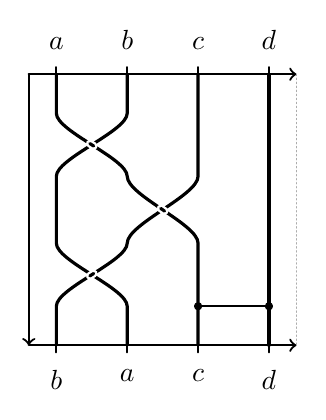
\begin{tikzpicture}[x=1cm,y=1cm,line cap=round,line join=round]
\coordinate (braid-base) at (1.35,-0.496);
\coordinate (braid-center) at (1.35,1.225);
\draw[draw=black,line width=0.8pt,->] (-0.35,2.946) -- (3.05,2.946);
\draw[draw=black,line width=0.8pt,->] (-0.35,-0.496) -- (3.05,-0.496);
\draw[draw=black,line width=0.8pt,->] (-0.35,2.946) -- (-0.35,-0.496);
\draw[gray!65,densely dotted,line width=0.45pt] (3.05,2.946) -- (3.05,-0.496);
\draw[draw=black,line width=0.8pt] (0,2.856) -- (0,3.036);
\draw[draw=black,line width=0.8pt] (0.9,2.856) -- (0.9,3.036);
\draw[draw=black,line width=0.8pt] (1.8,2.856) -- (1.8,3.036);
\draw[draw=black,line width=0.8pt] (2.7,2.856) -- (2.7,3.036);
\draw[draw=black,line width=0.8pt] (0,-0.586) -- (0,-0.406);
\draw[draw=black,line width=0.8pt] (0.9,-0.586) -- (0.9,-0.406);
\draw[draw=black,line width=0.8pt] (1.8,-0.586) -- (1.8,-0.406);
\draw[draw=black,line width=0.8pt] (2.7,-0.586) -- (2.7,-0.406);
\draw[draw=black,line width=0.75pt] (1.8,0) -- (2.7,0);
\draw[draw=black,line width=1.15pt,line cap=round,line join=round] (0,2.946) .. controls (0,2.75752) and (0,2.63848) .. (0,2.45) .. controls (0,2.222) and (0.9,1.878) .. (0.9,1.65) .. controls (0.9,1.40775) and (1.8,1.04225) .. (1.8,0.8) -- (1.8,0) .. controls (1.8,-0.18848) and (1.8,-0.30752) .. (1.8,-0.496);
\draw[draw=black,line width=1.15pt,line cap=round,line join=round] (0.9,2.946) .. controls (0.9,2.75752) and (0.9,2.63848) .. (0.9,2.45) .. controls (0.9,2.222) and (0,1.878) .. (0,1.65) -- (0,0.8) .. controls (0,0.572) and (0.9,0.228) .. (0.9,0) .. controls (0.9,-0.18848) and (0.9,-0.30752) .. (0.9,-0.496);
\draw[draw=black,line width=1.15pt,line cap=round,line join=round] (1.8,2.946) .. controls (1.8,2.75752) and (1.8,2.63848) .. (1.8,2.45) -- (1.8,1.65) .. controls (1.8,1.40775) and (0.9,1.04225) .. (0.9,0.8) .. controls (0.9,0.572) and (0,0.228) .. (0,0) .. controls (0,-0.18848) and (0,-0.30752) .. (0,-0.496);
\draw[draw=black,line width=1.15pt,line cap=round,line join=round] (2.7,2.946) .. controls (2.7,2.75752) and (2.7,2.63848) .. (2.7,2.45) -- (2.7,1.65) -- (2.7,0.8) -- (2.7,0) .. controls (2.7,-0.18848) and (2.7,-0.30752) .. (2.7,-0.496);
\draw[draw=white,line width=2.85pt,line cap=round,line join=round] (0.42571,2.06544) .. controls (0.44189,2.05515) and (0.45811,2.04485) .. (0.47429,2.03456);
\draw[draw=black,line width=1.15pt,line cap=round,line join=round] (0.42571,2.06544) .. controls (0.44189,2.05515) and (0.45811,2.04485) .. (0.47429,2.03456);
\draw[draw=white,line width=2.85pt,line cap=round,line join=round] (1.32571,1.24141) .. controls (1.34189,1.23047) and (1.35811,1.21953) .. (1.37429,1.20859);
\draw[draw=black,line width=1.15pt,line cap=round,line join=round] (1.32571,1.24141) .. controls (1.34189,1.23047) and (1.35811,1.21953) .. (1.37429,1.20859);
\draw[draw=white,line width=2.85pt,line cap=round,line join=round] (0.47429,0.41544) .. controls (0.45811,0.40515) and (0.44189,0.39485) .. (0.42571,0.38456);
\draw[draw=black,line width=1.15pt,line cap=round,line join=round] (0.47429,0.41544) .. controls (0.45811,0.40515) and (0.44189,0.39485) .. (0.42571,0.38456);
\fill[draw=black,fill=black] (1.8,0) circle[radius=0.045];
\fill[draw=black,fill=black] (2.7,0) circle[radius=0.045];
\node[inner sep=1pt,anchor=south] at (0,3.216) {$a$};
\node[inner sep=1pt,anchor=south] at (0.9,3.216) {$b$};
\node[inner sep=1pt,anchor=south] at (1.8,3.216) {$c$};
\node[inner sep=1pt,anchor=south] at (2.7,3.216) {$d$};
\node[inner sep=1pt,anchor=north] at (0,-0.766) {$b$};
\node[inner sep=1pt,anchor=north] at (0.9,-0.766) {$a$};
\node[inner sep=1pt,anchor=north] at (1.8,-0.766) {$c$};
\node[inner sep=1pt,anchor=north] at (2.7,-0.766) {$d$};
\end{tikzpicture}
}\end{center}
\smallskip
\needspace{6.3cm}
\textbf{Vertical stacking as model composition}\par
\smallskip
\begin{center}\resizebox{!}{5.0cm}{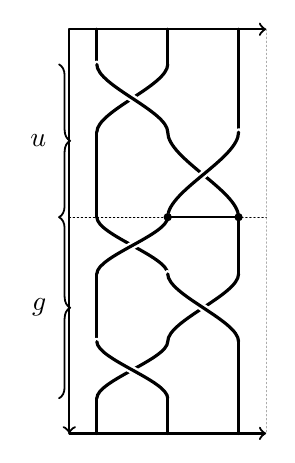
\begin{tikzpicture}[x=1cm,y=1cm,line cap=round,line join=round]
\coordinate (braid-base) at (0.9,-0.4464);
\draw[draw=black,line width=0.8pt,->] (-0.35,4.6864) -- (2.15,4.6864);
\draw[draw=black,line width=0.8pt,->] (-0.35,-0.4464) -- (2.15,-0.4464);
\draw[draw=black,line width=0.8pt,->] (-0.35,4.6864) -- (-0.35,-0.4464);
\draw[gray!65,densely dotted,line width=0.45pt] (2.15,4.6864) -- (2.15,-0.4464);
\draw[densely dotted,line width=0.45pt] (-0.35,2.3) -- (2.15,2.3);
\draw[draw=black,line width=1.15pt] (0,4.6864) .. controls (0,4.51677) and (0,4.40963) .. (0,4.24);
\draw[draw=black,line width=1.15pt] (0.9,4.6864) .. controls (0.9,4.51677) and (0.9,4.40963) .. (0.9,4.24);
\draw[draw=black,line width=1.15pt] (1.8,4.6864) .. controls (1.8,4.51677) and (1.8,4.40963) .. (1.8,4.24);
\draw[draw=black,line width=1.15pt] (1.8,4.24) -- (1.8,3.38);
\draw[draw=black,line width=1.15pt] (0.9,4.24) .. controls (0.9,3.9734) and (0,3.6466) .. (0,3.38);
\draw[draw=white,line width=2.85pt] (0,4.24) .. controls (0,3.9734) and (0.9,3.6466) .. (0.9,3.38);
\draw[draw=black,line width=1.15pt] (0,4.24) .. controls (0,3.9734) and (0.9,3.6466) .. (0.9,3.38);
\draw[draw=black,line width=1.15pt] (0,3.38) -- (0,2.3);
\draw[draw=black,line width=1.15pt] (0.9,3.38) .. controls (0.9,3.0452) and (1.8,2.6348) .. (1.8,2.3);
\draw[draw=white,line width=2.85pt] (1.8,3.38) .. controls (1.8,3.0452) and (0.9,2.6348) .. (0.9,2.3);
\draw[draw=black,line width=1.15pt] (1.8,3.38) .. controls (1.8,3.0452) and (0.9,2.6348) .. (0.9,2.3);
\draw[draw=black,line width=1.15pt] (1.8,2.3) -- (1.8,1.58);
\draw[draw=black,line width=1.15pt] (0,2.3) .. controls (0,2.0768) and (0.9,1.8032) .. (0.9,1.58);
\draw[draw=white,line width=2.85pt] (0.9,2.3) .. controls (0.9,2.0768) and (0,1.8032) .. (0,1.58);
\draw[draw=black,line width=1.15pt] (0.9,2.3) .. controls (0.9,2.0768) and (0,1.8032) .. (0,1.58);
\draw[draw=black,line width=1.15pt] (0,1.58) -- (0,0.72);
\draw[draw=black,line width=1.15pt] (1.8,1.58) .. controls (1.8,1.3134) and (0.9,0.9866) .. (0.9,0.72);
\draw[draw=white,line width=2.85pt] (0.9,1.58) .. controls (0.9,1.3134) and (1.8,0.9866) .. (1.8,0.72);
\draw[draw=black,line width=1.15pt] (0.9,1.58) .. controls (0.9,1.3134) and (1.8,0.9866) .. (1.8,0.72);
\draw[draw=black,line width=1.15pt] (1.8,0.72) -- (1.8,0);
\draw[draw=black,line width=1.15pt] (0.9,0.72) .. controls (0.9,0.4968) and (0,0.2232) .. (0,0);
\draw[draw=white,line width=2.85pt] (0,0.72) .. controls (0,0.4968) and (0.9,0.2232) .. (0.9,0);
\draw[draw=black,line width=1.15pt] (0,0.72) .. controls (0,0.4968) and (0.9,0.2232) .. (0.9,0);
\draw[draw=black,line width=1.15pt] (0,0) .. controls (0,-0.16963) and (0,-0.27677) .. (0,-0.4464);
\draw[draw=black,line width=1.15pt] (0.9,0) .. controls (0.9,-0.16963) and (0.9,-0.27677) .. (0.9,-0.4464);
\draw[draw=black,line width=1.15pt] (1.8,0) .. controls (1.8,-0.16963) and (1.8,-0.27677) .. (1.8,-0.4464);
\draw[draw=black,line width=0.75pt] (1.8,2.3) -- (0.9,2.3);
\fill[draw=black,fill=black] (1.8,2.3) circle[radius=0.045];
\fill[draw=black,fill=black] (0.9,2.3) circle[radius=0.045];
\draw[decorate,decoration={brace,amplitude=4pt},draw=black,line width=0.65pt] (-0.48,4.24) -- (-0.48,2.3);
\node[anchor=east,inner sep=1pt] at (-0.6,3.27) {$u$};
\draw[decorate,decoration={brace,amplitude=4pt},draw=black,line width=0.65pt] (-0.48,2.3) -- (-0.48,0);
\node[anchor=east,inner sep=1pt] at (-0.6,1.15) {$g$};
\end{tikzpicture}
}\end{center}
\smallskip
\needspace{6.3cm}
\textbf{Operadic strand replacement: connector alternatives}\par
\smallskip
\begin{center}\resizebox{!}{4.2cm}{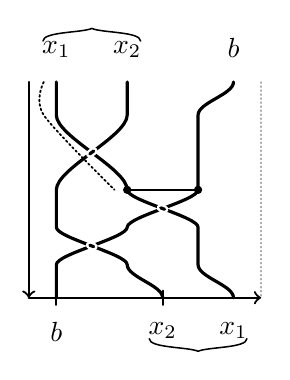
\begin{tikzpicture}[x=1cm,y=1cm,line cap=round,line join=round]
\coordinate (braid-base) at (1.125,-0.42);
\coordinate (braid-center) at (1.125,0.95);
\draw[draw=black,line width=0.8pt,->] (-0.35,-0.42) -- (2.6,-0.42);
\draw[draw=black,line width=0.8pt,->] (-0.35,2.32) -- (-0.35,-0.42);
\draw[gray!65,densely dotted,line width=0.45pt] (2.6,2.32) -- (2.6,-0.42);
\draw[draw=black,line width=0.8pt] (0,-0.51) -- (0,-0.33);
\draw[draw=black,line width=0.8pt] (1.35,-0.51) -- (1.35,-0.33);
\draw[draw=black,line width=0.75pt] (0.9,0.95) -- (1.8,0.95);
\draw[draw=black,line width=1.15pt,line cap=round,line join=round] (0,2.32) .. controls (0,2.1604) and (0,2.0596) .. (0,1.9) .. controls (0,1.62925) and (0.9,1.22075) .. (0.9,0.95) .. controls (0.9,0.81462) and (1.8,0.61038) .. (1.8,0.475) -- (1.8,0) .. controls (1.8,-0.1596) and (2.25,-0.2604) .. (2.25,-0.42);
\draw[draw=black,line width=1.15pt,line cap=round,line join=round] (0.9,2.32) .. controls (0.9,2.1604) and (0.9,2.0596) .. (0.9,1.9) .. controls (0.9,1.62925) and (0,1.22075) .. (0,0.95) -- (0,0.475) .. controls (0,0.33962) and (0.9,0.13537) .. (0.9,0) .. controls (0.9,-0.1596) and (1.35,-0.2604) .. (1.35,-0.42);
\draw[draw=black,line width=1.15pt,line cap=round,line join=round] (2.25,2.32) .. controls (2.25,2.1604) and (1.8,2.0596) .. (1.8,1.9) -- (1.8,0.95) .. controls (1.8,0.81462) and (0.9,0.61038) .. (0.9,0.475) .. controls (0.9,0.33962) and (0,0.13537) .. (0,0) .. controls (0,-0.1596) and (0,-0.2604) .. (0,-0.42);
\draw[draw=white,line width=2.85pt,line cap=round,line join=round] (0.47429,1.44334) .. controls (0.45811,1.43111) and (0.44189,1.41889) .. (0.42571,1.40666);
\draw[draw=black,line width=1.15pt,line cap=round,line join=round] (0.47429,1.44334) .. controls (0.45811,1.43111) and (0.44189,1.41889) .. (0.42571,1.40666);
\draw[draw=white,line width=2.85pt,line cap=round,line join=round] (1.32571,0.72167) .. controls (1.34189,0.71556) and (1.35811,0.70944) .. (1.37429,0.70333);
\draw[draw=black,line width=1.15pt,line cap=round,line join=round] (1.32571,0.72167) .. controls (1.34189,0.71556) and (1.35811,0.70944) .. (1.37429,0.70333);
\draw[draw=white,line width=2.85pt,line cap=round,line join=round] (0.42571,0.24667) .. controls (0.44189,0.24056) and (0.45811,0.23444) .. (0.47429,0.22833);
\draw[draw=black,line width=1.15pt,line cap=round,line join=round] (0.42571,0.24667) .. controls (0.44189,0.24056) and (0.45811,0.23444) .. (0.47429,0.22833);
\fill[draw=black,fill=black] (0.9,0.95) circle[radius=0.045];
\fill[draw=black,fill=black] (1.8,0.95) circle[radius=0.045];
\draw[draw=black,line width=0.65pt,densely dotted,line cap=round,line join=round] plot[smooth] coordinates {(-0.16,2.32) (-0.16,1.9) (0.74,0.95)};
\node[inner sep=1pt,anchor=south] at (0,2.59) {$x_1$};
\node[inner sep=1pt,anchor=south] at (0.9,2.59) {$x_2$};
\node[inner sep=1pt,anchor=south] at (2.25,2.59) {$b$};
\node[inner sep=1pt,anchor=north] at (0,-0.69) {$b$};
\node[inner sep=1pt,anchor=north] at (1.35,-0.69) {$x_2$};
\node[inner sep=1pt,anchor=north] at (2.25,-0.69) {$x_1$};
\draw[line width=0.55pt] (-0.17,2.84) .. controls (-0.17,2.96) and (0.326,2.944) .. (0.45,3) .. controls (0.574,2.944) and (1.07,2.96) .. (1.07,2.84);
\draw[line width=0.55pt] (1.18,-0.94) .. controls (1.18,-1.06) and (1.676,-1.044) .. (1.8,-1.1) .. controls (1.924,-1.044) and (2.42,-1.06) .. (2.42,-0.94);
\end{tikzpicture}
}\quad$+$\quad\resizebox{!}{4.2cm}{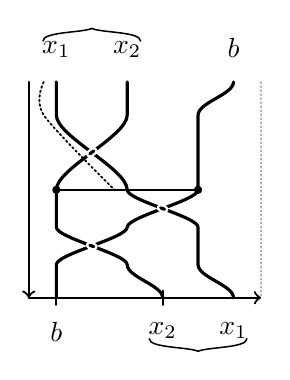
\begin{tikzpicture}[x=1cm,y=1cm,line cap=round,line join=round]
\coordinate (braid-base) at (1.125,-0.42);
\coordinate (braid-center) at (1.125,0.95);
\draw[draw=black,line width=0.8pt,->] (-0.35,-0.42) -- (2.6,-0.42);
\draw[draw=black,line width=0.8pt,->] (-0.35,2.32) -- (-0.35,-0.42);
\draw[gray!65,densely dotted,line width=0.45pt] (2.6,2.32) -- (2.6,-0.42);
\draw[draw=black,line width=0.8pt] (0,-0.51) -- (0,-0.33);
\draw[draw=black,line width=0.8pt] (1.35,-0.51) -- (1.35,-0.33);
\draw[draw=black,line width=0.75pt] (0,0.95) -- (1.8,0.95);
\draw[draw=black,line width=1.15pt,line cap=round,line join=round] (0,2.32) .. controls (0,2.1604) and (0,2.0596) .. (0,1.9) .. controls (0,1.62925) and (0.9,1.22075) .. (0.9,0.95) .. controls (0.9,0.81462) and (1.8,0.61038) .. (1.8,0.475) -- (1.8,0) .. controls (1.8,-0.1596) and (2.25,-0.2604) .. (2.25,-0.42);
\draw[draw=black,line width=1.15pt,line cap=round,line join=round] (0.9,2.32) .. controls (0.9,2.1604) and (0.9,2.0596) .. (0.9,1.9) .. controls (0.9,1.62925) and (0,1.22075) .. (0,0.95) -- (0,0.475) .. controls (0,0.33962) and (0.9,0.13537) .. (0.9,0) .. controls (0.9,-0.1596) and (1.35,-0.2604) .. (1.35,-0.42);
\draw[draw=black,line width=1.15pt,line cap=round,line join=round] (2.25,2.32) .. controls (2.25,2.1604) and (1.8,2.0596) .. (1.8,1.9) -- (1.8,0.95) .. controls (1.8,0.81462) and (0.9,0.61038) .. (0.9,0.475) .. controls (0.9,0.33962) and (0,0.13537) .. (0,0) .. controls (0,-0.1596) and (0,-0.2604) .. (0,-0.42);
\draw[draw=white,line width=2.85pt,line cap=round,line join=round] (0.47429,1.44334) .. controls (0.45811,1.43111) and (0.44189,1.41889) .. (0.42571,1.40666);
\draw[draw=black,line width=1.15pt,line cap=round,line join=round] (0.47429,1.44334) .. controls (0.45811,1.43111) and (0.44189,1.41889) .. (0.42571,1.40666);
\draw[draw=white,line width=2.85pt,line cap=round,line join=round] (1.32571,0.72167) .. controls (1.34189,0.71556) and (1.35811,0.70944) .. (1.37429,0.70333);
\draw[draw=black,line width=1.15pt,line cap=round,line join=round] (1.32571,0.72167) .. controls (1.34189,0.71556) and (1.35811,0.70944) .. (1.37429,0.70333);
\draw[draw=white,line width=2.85pt,line cap=round,line join=round] (0.42571,0.24667) .. controls (0.44189,0.24056) and (0.45811,0.23444) .. (0.47429,0.22833);
\draw[draw=black,line width=1.15pt,line cap=round,line join=round] (0.42571,0.24667) .. controls (0.44189,0.24056) and (0.45811,0.23444) .. (0.47429,0.22833);
\fill[draw=black,fill=black] (0,0.95) circle[radius=0.045];
\fill[draw=black,fill=black] (1.8,0.95) circle[radius=0.045];
\draw[draw=black,line width=0.65pt,densely dotted,line cap=round,line join=round] plot[smooth] coordinates {(-0.16,2.32) (-0.16,1.9) (0.74,0.95)};
\node[inner sep=1pt,anchor=south] at (0,2.59) {$x_1$};
\node[inner sep=1pt,anchor=south] at (0.9,2.59) {$x_2$};
\node[inner sep=1pt,anchor=south] at (2.25,2.59) {$b$};
\node[inner sep=1pt,anchor=north] at (0,-0.69) {$b$};
\node[inner sep=1pt,anchor=north] at (1.35,-0.69) {$x_2$};
\node[inner sep=1pt,anchor=north] at (2.25,-0.69) {$x_1$};
\draw[line width=0.55pt] (-0.17,2.84) .. controls (-0.17,2.96) and (0.326,2.944) .. (0.45,3) .. controls (0.574,2.944) and (1.07,2.96) .. (1.07,2.84);
\draw[line width=0.55pt] (1.18,-0.94) .. controls (1.18,-1.06) and (1.676,-1.044) .. (1.8,-1.1) .. controls (1.924,-1.044) and (2.42,-1.06) .. (2.42,-0.94);
\end{tikzpicture}
}\end{center}
\smallskip
\needspace{6.3cm}
\textbf{Four strands, connectors, separator, and regions}\par
\smallskip
\begin{center}\resizebox{!}{5.0cm}{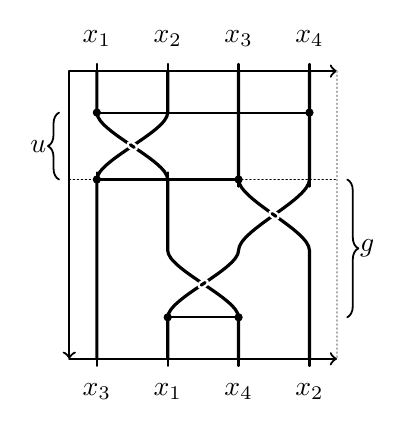
\begin{tikzpicture}[x=1cm,y=1cm,line cap=round,line join=round]
\coordinate (braid-base) at (1.35,-0.527);
\coordinate (braid-center) at (1.35,1.3);
\draw[draw=black,line width=0.8pt,->] (-0.35,3.127) -- (3.05,3.127);
\draw[draw=black,line width=0.8pt,->] (-0.35,-0.527) -- (3.05,-0.527);
\draw[draw=black,line width=0.8pt,->] (-0.35,3.127) -- (-0.35,-0.527);
\draw[gray!65,densely dotted,line width=0.45pt] (3.05,3.127) -- (3.05,-0.527);
\draw[draw=black,line width=0.8pt] (0,3.037) -- (0,3.217);
\draw[draw=black,line width=0.8pt] (0.9,3.037) -- (0.9,3.217);
\draw[draw=black,line width=0.8pt] (1.8,3.037) -- (1.8,3.217);
\draw[draw=black,line width=0.8pt] (2.7,3.037) -- (2.7,3.217);
\draw[draw=black,line width=0.8pt] (0,-0.617) -- (0,-0.437);
\draw[draw=black,line width=0.8pt] (0.9,-0.617) -- (0.9,-0.437);
\draw[draw=black,line width=0.8pt] (1.8,-0.617) -- (1.8,-0.437);
\draw[draw=black,line width=0.8pt] (2.7,-0.617) -- (2.7,-0.437);
\draw[densely dotted,line width=0.45pt] (-0.35,1.75) -- (3.05,1.75);
\draw[draw=black,line width=0.8pt] (0,1.66) -- (0,1.84);
\draw[draw=black,line width=0.8pt] (0.9,1.66) -- (0.9,1.84);
\draw[draw=black,line width=0.8pt] (1.8,1.66) -- (1.8,1.84);
\draw[draw=black,line width=0.8pt] (2.7,1.66) -- (2.7,1.84);
\draw[draw=black,line width=0.75pt] (0,2.6) -- (2.7,2.6);
\draw[draw=black,line width=0.75pt] (0,1.75) -- (1.8,1.75);
\draw[draw=black,line width=0.75pt] (1.8,0) -- (0.9,0);
\draw[draw=black,line width=1.15pt,line cap=round,line join=round] (0,3.127) .. controls (0,2.92674) and (0,2.80026) .. (0,2.6) .. controls (0,2.35775) and (0.9,1.99225) .. (0.9,1.75) -- (0.9,0.85) .. controls (0.9,0.60775) and (1.8,0.24225) .. (1.8,0) .. controls (1.8,-0.20026) and (1.8,-0.32674) .. (1.8,-0.527);
\draw[draw=black,line width=1.15pt,line cap=round,line join=round] (0.9,3.127) .. controls (0.9,2.92674) and (0.9,2.80026) .. (0.9,2.6) .. controls (0.9,2.35775) and (0,1.99225) .. (0,1.75) -- (0,0.85) -- (0,0) .. controls (0,-0.20026) and (0,-0.32674) .. (0,-0.527);
\draw[draw=black,line width=1.15pt,line cap=round,line join=round] (1.8,3.127) .. controls (1.8,2.92674) and (1.8,2.80026) .. (1.8,2.6) -- (1.8,1.75) .. controls (1.8,1.4935) and (2.7,1.1065) .. (2.7,0.85) -- (2.7,0) .. controls (2.7,-0.20026) and (2.7,-0.32674) .. (2.7,-0.527);
\draw[draw=black,line width=1.15pt,line cap=round,line join=round] (2.7,3.127) .. controls (2.7,2.92674) and (2.7,2.80026) .. (2.7,2.6) -- (2.7,1.75) .. controls (2.7,1.4935) and (1.8,1.1065) .. (1.8,0.85) .. controls (1.8,0.60775) and (0.9,0.24225) .. (0.9,0) .. controls (0.9,-0.20026) and (0.9,-0.32674) .. (0.9,-0.527);
\draw[draw=white,line width=2.85pt,line cap=round,line join=round] (0.42571,2.19141) .. controls (0.44189,2.18047) and (0.45811,2.16953) .. (0.47429,2.15859);
\draw[draw=black,line width=1.15pt,line cap=round,line join=round] (0.42571,2.19141) .. controls (0.44189,2.18047) and (0.45811,2.16953) .. (0.47429,2.15859);
\draw[draw=white,line width=2.85pt,line cap=round,line join=round] (2.22571,1.31737) .. controls (2.24189,1.30579) and (2.25811,1.29421) .. (2.27429,1.28263);
\draw[draw=black,line width=1.15pt,line cap=round,line join=round] (2.22571,1.31737) .. controls (2.24189,1.30579) and (2.25811,1.29421) .. (2.27429,1.28263);
\draw[draw=white,line width=2.85pt,line cap=round,line join=round] (1.37429,0.44141) .. controls (1.35811,0.43047) and (1.34189,0.41953) .. (1.32571,0.40859);
\draw[draw=black,line width=1.15pt,line cap=round,line join=round] (1.37429,0.44141) .. controls (1.35811,0.43047) and (1.34189,0.41953) .. (1.32571,0.40859);
\fill[draw=black,fill=black] (0,2.6) circle[radius=0.045];
\fill[draw=black,fill=black] (2.7,2.6) circle[radius=0.045];
\fill[draw=black,fill=black] (0,1.75) circle[radius=0.045];
\fill[draw=black,fill=black] (1.8,1.75) circle[radius=0.045];
\fill[draw=black,fill=black] (1.8,0) circle[radius=0.045];
\fill[draw=black,fill=black] (0.9,0) circle[radius=0.045];
\draw[decorate,decoration={brace,amplitude=4pt,mirror},draw=black,line width=0.65pt] (-0.48,2.6) -- (-0.48,1.75);
\node[anchor=east,inner sep=1pt] at (-0.6,2.175) {$u$};
\draw[decorate,decoration={brace,amplitude=4pt},draw=black,line width=0.65pt] (3.18,1.75) -- (3.18,0);
\node[anchor=west,inner sep=1pt] at (3.3,0.875) {$g$};
\node[inner sep=1pt,anchor=south] at (0,3.397) {$x_1$};
\node[inner sep=1pt,anchor=south] at (0.9,3.397) {$x_2$};
\node[inner sep=1pt,anchor=south] at (1.8,3.397) {$x_3$};
\node[inner sep=1pt,anchor=south] at (2.7,3.397) {$x_4$};
\node[inner sep=1pt,anchor=north] at (0,-0.797) {$x_3$};
\node[inner sep=1pt,anchor=north] at (0.9,-0.797) {$x_1$};
\node[inner sep=1pt,anchor=north] at (1.8,-0.797) {$x_4$};
\node[inner sep=1pt,anchor=north] at (2.7,-0.797) {$x_2$};
\end{tikzpicture}
}\end{center}
\smallskip
\needspace{6.3cm}
\textbf{Repeated crossings and dotted auxiliary paths}\par
\smallskip
\begin{center}\resizebox{!}{5.0cm}{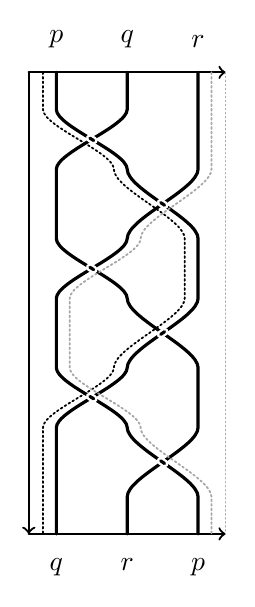
\begin{tikzpicture}[x=1cm,y=1cm,line cap=round,line join=round]
\coordinate (braid-base) at (0.9,-0.4712);
\coordinate (braid-center) at (0.9,2.46);
\draw[draw=black,line width=0.8pt,->] (-0.35,5.3912) -- (2.15,5.3912);
\draw[draw=black,line width=0.8pt,->] (-0.35,-0.4712) -- (2.15,-0.4712);
\draw[draw=black,line width=0.8pt,->] (-0.35,5.3912) -- (-0.35,-0.4712);
\draw[gray!65,densely dotted,line width=0.45pt] (2.15,5.3912) -- (2.15,-0.4712);
\draw[draw=black,line width=1.15pt,line cap=round,line join=round] (0,5.3912) .. controls (0,5.21214) and (0,5.09906) .. (0,4.92) .. controls (0,4.7034) and (0.9,4.3766) .. (0.9,4.16) .. controls (0.9,3.9092) and (1.8,3.5308) .. (1.8,3.28) -- (1.8,2.52) .. controls (1.8,2.2692) and (0.9,1.8908) .. (0.9,1.64) .. controls (0.9,1.4234) and (0,1.0966) .. (0,0.88) -- (0,0) .. controls (0,-0.17906) and (0,-0.29214) .. (0,-0.4712);
\draw[draw=black,line width=1.15pt,line cap=round,line join=round] (0.9,5.3912) .. controls (0.9,5.21214) and (0.9,5.09906) .. (0.9,4.92) .. controls (0.9,4.7034) and (0,4.3766) .. (0,4.16) -- (0,3.28) .. controls (0,3.0634) and (0.9,2.7366) .. (0.9,2.52) .. controls (0.9,2.2692) and (1.8,1.8908) .. (1.8,1.64) -- (1.8,0.88) .. controls (1.8,0.6292) and (0.9,0.2508) .. (0.9,0) .. controls (0.9,-0.17906) and (0.9,-0.29214) .. (0.9,-0.4712);
\draw[draw=black,line width=1.15pt,line cap=round,line join=round] (1.8,5.3912) .. controls (1.8,5.21214) and (1.8,5.09906) .. (1.8,4.92) -- (1.8,4.16) .. controls (1.8,3.9092) and (0.9,3.5308) .. (0.9,3.28) .. controls (0.9,3.0634) and (0,2.7366) .. (0,2.52) -- (0,1.64) .. controls (0,1.4234) and (0.9,1.0966) .. (0.9,0.88) .. controls (0.9,0.6292) and (1.8,0.2508) .. (1.8,0) .. controls (1.8,-0.17906) and (1.8,-0.29214) .. (1.8,-0.4712);
\draw[draw=white,line width=2.85pt,line cap=round,line join=round] (0.42571,4.55467) .. controls (0.44189,4.54489) and (0.45811,4.53511) .. (0.47429,4.52533);
\draw[draw=black,line width=1.15pt,line cap=round,line join=round] (0.42571,4.55467) .. controls (0.44189,4.54489) and (0.45811,4.53511) .. (0.47429,4.52533);
\draw[draw=white,line width=2.85pt,line cap=round,line join=round] (1.32571,3.73699) .. controls (1.34189,3.72566) and (1.35811,3.71434) .. (1.37429,3.70301);
\draw[draw=black,line width=1.15pt,line cap=round,line join=round] (1.32571,3.73699) .. controls (1.34189,3.72566) and (1.35811,3.71434) .. (1.37429,3.70301);
\draw[draw=white,line width=2.85pt,line cap=round,line join=round] (0.42571,2.91467) .. controls (0.44189,2.90489) and (0.45811,2.89511) .. (0.47429,2.88533);
\draw[draw=black,line width=1.15pt,line cap=round,line join=round] (0.42571,2.91467) .. controls (0.44189,2.90489) and (0.45811,2.89511) .. (0.47429,2.88533);
\draw[draw=white,line width=2.85pt,line cap=round,line join=round] (1.37429,2.09699) .. controls (1.35811,2.08566) and (1.34189,2.07434) .. (1.32571,2.06301);
\draw[draw=black,line width=1.15pt,line cap=round,line join=round] (1.37429,2.09699) .. controls (1.35811,2.08566) and (1.34189,2.07434) .. (1.32571,2.06301);
\draw[draw=white,line width=2.85pt,line cap=round,line join=round] (0.42571,1.27467) .. controls (0.44189,1.26489) and (0.45811,1.25511) .. (0.47429,1.24533);
\draw[draw=black,line width=1.15pt,line cap=round,line join=round] (0.42571,1.27467) .. controls (0.44189,1.26489) and (0.45811,1.25511) .. (0.47429,1.24533);
\draw[draw=white,line width=2.85pt,line cap=round,line join=round] (1.32571,0.45699) .. controls (1.34189,0.44566) and (1.35811,0.43434) .. (1.37429,0.42301);
\draw[draw=black,line width=1.15pt,line cap=round,line join=round] (1.32571,0.45699) .. controls (1.34189,0.44566) and (1.35811,0.43434) .. (1.37429,0.42301);
\draw[draw=black,line width=0.65pt,densely dotted,line cap=round,line join=round] (-0.17,5.3912) .. controls (-0.17,5.21214) and (-0.17,5.09906) .. (-0.17,4.92) .. controls (-0.17,4.7034) and (0.73,4.3766) .. (0.73,4.16) .. controls (0.73,3.9092) and (1.63,3.5308) .. (1.63,3.28) -- (1.63,2.52) .. controls (1.63,2.2692) and (0.73,1.8908) .. (0.73,1.64) .. controls (0.73,1.4234) and (-0.17,1.0966) .. (-0.17,0.88) -- (-0.17,0) .. controls (-0.17,-0.17906) and (-0.17,-0.29214) .. (-0.17,-0.4712);
\draw[draw=gray!70,line width=0.65pt,densely dotted,line cap=round,line join=round] (1.97,5.3912) .. controls (1.97,5.21214) and (1.97,5.09906) .. (1.97,4.92) -- (1.97,4.16) .. controls (1.97,3.9092) and (1.07,3.5308) .. (1.07,3.28) .. controls (1.07,3.0634) and (0.17,2.7366) .. (0.17,2.52) -- (0.17,1.64) .. controls (0.17,1.4234) and (1.07,1.0966) .. (1.07,0.88) .. controls (1.07,0.6292) and (1.97,0.2508) .. (1.97,0) .. controls (1.97,-0.17906) and (1.97,-0.29214) .. (1.97,-0.4712);
\node[inner sep=1pt,anchor=south] at (0,5.6612) {$p$};
\node[inner sep=1pt,anchor=south] at (0.9,5.6612) {$q$};
\node[inner sep=1pt,anchor=south] at (1.8,5.6612) {$r$};
\node[inner sep=1pt,anchor=north] at (0,-0.7412) {$q$};
\node[inner sep=1pt,anchor=north] at (0.9,-0.7412) {$r$};
\node[inner sep=1pt,anchor=north] at (1.8,-0.7412) {$p$};
\end{tikzpicture}
}\end{center}
\smallskip
\end{document}
